%%%%%%%%%%%%%%%%%%%%%%%%%%%%%%%%%%%%%%%%%%%%%%%%%%%%%%%%%%%%%%%%%%%%%%%%%%%%%
%% Descr:       Vorlage für Berichte der DHBW-Karlsruhe, Ein Kapitel
%% Author:      Prof. Dr. Jürgen Vollmer, vollmer@dhbw-karlsruhe.de
%% $Id: kapitel2.tex,v 1.5 2017/10/06 14:02:51 vollmer Exp $
%%  -*- coding: utf-8 -*-
%%%%%%%%%%%%%%%%%%%%%%%%%%%%%%%%%%%%%%%%%%%%%%%%%%%%%%%%%%%%%%%%%%%%%%%%%%%%%%%

\chapter{Grundlagen}
\label{chap:Grundlagen}
In diesem Kapitel werden die für diese Bachelorarbeit notwendigen Grundlagen geschaffen, um ein fundiertes Wissen und Verständnis 
über verwendete Technologien zu bilden. Auf alle diese Informationen und Voraussetzungen wird im Folgenden eingegangen, um nachfolgende 
Konzeption und Umsetzung besser zu verstehen.

\section{Augmented Reality}
\label{chap:Augmented Reality}
Eine der wichtigsten Grundlagen dieser Arbeit ist das Verständnis des Begriffs der Augmented Reality.
\\ 
\acl{AR}, im Deutschen \textit{„erweiterte Realität“}, ist eine durch den Computer gestützte Erweiterung der Realität, bzw. der menschlichen 
Wahrnehmung. Es ermöglicht dem Nutzer, die reale Welt mit Überlagerung oder Zusammensetzung virtueller Objekte und visueller Informationen
zu sehen. Mittels einer Art Overlay werden diese Objekte und Informationen über die reale Welt gelegt und dem Nutzer zur Verfügung gestellt. 
Allgemein soll damit dem Nutzer ein weit gefächerter Überblick verschafft und Hilfestellung geleistet werden, aihn aber in keinerlei 
Interaktion mit der Umgebung einschränken. Die Definition, welche sich in der Wissenschaft weitestgehend durchgesetzt und etabliert hat, ist 
die Definition nach Azuma aus dem Jahre 1997.
\begin{quote}
    „Augmented Reality (AR) is a variation of Virtual Environments (VE), or Virtual Reality as it is more commonly called. VE 
    technologies completely immerse a user inside a synthetic environment. While immersed, the user cannot see the real world around him. 
    In contrast, AR allows the user to see the real world, with virtual objects superimposed upon or composited with the real world. 
    Therefore, AR supplements reality, rather than completely replacing it.“ \cite{azuma.1997a}
\end{quote}
Ein Augmented Reality System verfügt nach \cite{azuma.1997a} über folgende drei charakteristische Merkmale: 
\begin{enumerate}
    \item Es kombiniert Realität und Virtualität.
    \item Es ist interaktiv in Echtzeit.
    \item Die virtuellen Inhalte sind im 3D registriert.
\end{enumerate}
Das erste genannte Merkmal kombiniert die reale Welt mit dem oben genannten Overlay, der Überlagerung der Realität, um künstliche virtuelle 
Objekte und visuelle Informationen darstellen zu können. Dies bedeutet, der Nutzer nimmt die reale Umgebung gleichzeitig mit den darin liegenden virtuellen 
Objekten als ein Ganzes wahr. Daraus resultiert die Interaktion von virtuellen Objekten und Informationen mit der realen Welt in Echtzeit, 
damit sie als Teil der Realität registriert werden können. Das dritte Merkmal umfasst die Darstellung von Objekten als scheinbar reales 
Objekt. Mit dem letzt genannten Merkmal wird das Ziel verfolgt die projizierten, bzw. nicht realen Teile täuschend echt in die Umgebung zu 
integrieren.
\\ 
\linebreak  
%Darüber hinaus sind die virtuellen Inhalte in 3D (d. h. geometrisch) registriert. Dies bedeutet nichts anderes, als dass in einer 
%AR-Umgebung ein virtuelles Objekt scheinbar einen festen Platz in Realität hat und diesen, sofern es nicht durch eine Benutzerinteraktion 
%verändert wird oder sich z. B. in Form einer Animation selbst verändert, auch beibehält. Mit anderen Worten: Es verhält sich aus Nutzersicht 
%genauso, wie ein reales Objekt, was sich an diesem Ort befinden würde
Eine etwas allgemein formuliertere Definition ist die nach \cite{springer.2019s}, welche die drei charakteristischen Merkmale besonders 
aufgreift:
\begin{quote}
    „Augmentierte Realität (AR) ist eine (unmittelbare und interaktive) um virtuelle Inhalte (für beliebige Sinne) angereicherte Wahrnehmung der 
    realen Umgebung in Echtzeit, welche sich in ihrer Ausprägung und Anmutung soweit wie möglich an der Realität orientiert, sodass im 
    Extremfall (so dies gewünscht ist) eine Unterscheidung zwischen realen und virtuellen (Sinnes-) Eindrücken nicht mehr möglich ist.„ \cite{springer.2019s}
\end{quote}
%Diese Definition nimmt sich als Grundlage die oben aufgeführte Definition nach \cite{azuma.1997a}.
Die oben aufgeführte Definition von Azuma dient Dörner als Grundlage.
\\ 
\linebreak
Der Autor L. Frank Baum \cite{frankbaum.1856m} verkündete die ersten Ideen und Gedanken einer Augmented Reality Anwendung in 
\textit{„The Master Key“} \cite{masterkey.1996f}. Eine erste tatsächliche Realisierung eines Augmented Reality Systems erfolgte erst über 
60 Jahre später. Ivan Edward Sutherland \cite{sutherlandbio.1938m} stellte sein Projekt 1968 an der University of Utah vor. Dabei handelte es 
sich um ein sogenanntes \textit{\ac{HMD}}. Ziel dieser Entwicklung war weniger das Erweitern der Realität, sondern viel mehr das Erzeugen dreidimensionaler 
Illusionen, die reale Objekte mit einer einfachen Grafik in Echtzeit überlagern. %\cite{display.1965f}
Er gilt nichtsdestotrotz als erste Person mit der Vision, einen Nutzer in realer Umgebung mit virtuellen Objekten interagieren zu lassen.
\\ 
Anfang der 90er Jahre prägten zwei Forscher, Thomas P. Caudell und David W. Mizell, den Begriff der Augmented Reality durch ein Pilotprojekt
bei Boeing. Das Projekt diente dazu, Informationen in das Gesichtsfeld über eine Brille einzusetzen, um Arbeitern das Verlegen von Kabeln im und um das 
Flugzeug zu erleichtern. Nach dieser bahnbrechenden Erfindung begann eine stetige Weiterentwicklung der Technologie. Im Jahre 1999 wurde 
von Hirokazu Kato und Mark Billinghurst \textit{ARToolKit}, ein Computer-Vision-basiertes Tracking für AR, veröffentlicht und „löste eine 
große Welle an Forschungsarbeiten auf der ganzen Welt aus.“ \cite{springer.2019s} 
\begin{quote}
    We describe an augmented reality conferencing system which uses the overlay of virtual images on the real world. Remote collaborators 
    are represented on Virtual Monitors which can be freely positioned about a user in space. Users can collaboratively view and interact 
    with virtual objects using a shared virtual whiteboard. This is possible through precise virtual image registration using fast and 
    accurate computer vision techniques and HMD calibration. We propose a method for tracking fiducial markers and a calibration method 
    for optical see-through HMD based on the marker tracking. \cite{artoolkitsheet.1999o}
\end{quote}
Dieser Ausschnitt war der grundlegende Baustein des Durchbruchs dieser Technologie und den vorangestellten Forschungen und eine fundierte 
Grundlage für alle weiteren Forschungen und Entwicklungen, die darauf folgten. 
\\ 
Heutzutage dreht sich die Entwicklung vielmehr um mobile AR, welche durch die anfängliche Revolution von \textit{ARToolkit} und die darauf 
entstehenden Entwicklungen und Produktionen von großen Firmen, wie z.B. Google, Microsoft, Apple und Facebook entstand. Die zuletzt große 
Bewegung in dem Bereich der AR waren die Vorstellungen großer Software-Plattformen für mobile \acs{AR}-Applikationen, z.B. \acl{WMR}. Durch 
\textit{Apple's ARKit} und \textit{Google's ARCore} kamen im Jahr 2017 zwei moderne und innovative Frameworks auf den Markt, die die 
Entwicklung von \acl{AR}-Applikationen stark beeinflussen.Die Frameworks wurden bei den ersten Produktionen für Entertainment-Anwendungen 
genutzt, um z.B. mobile Spiele zur Unterhaltung oder Funktionen bei Sport-Fernsehübertragungen zur Anzeige der Entfernung des Freistoßes zu 
realisieren.
\\ 
\linebreak
%Dies ist hier nur nebenbei erwähnt. Ich möchte mich an dieser Stelle
Diese Arbeit widmet sich ausschließlich dem industriellen Aspekt und stellt andere Bereiche der \acl{AR} in den Hintergrund.
%Diese Arbeit jedoch widmet sich ausschließlich dem industriellen Aspekt und stellt andere Bereiche in den Hintergrund. 
Die schon in Kapitel (\ref{chap:Motivation}) aufgeführte Markstudie bestätigt das enorme Potential hinter \acl{AR} und deren Einsetzbarkeit 
in der Industrie. Hauptsächlich in der Produktion, der Wartung oder der Reparatur von Maschinen kann Augmentierte Realität eingesetzt werden 
und zeigt einen positiv erzeugten Mehrwert. Dabei können bei Maschinen das Anzeigen von protokollierten Fehlern oder eine visuelle 
Hilfestellung bei Defekts, sowohl bei der Reparatur, als auch bei der Ersetzung einzelner Komponenten eine deutliche Reduzierung des 
zeitlichen Aufwands oder eine effektivere Arbeitsweise vorweisen. 
\\
\textit{Harvard Business Review} legte einen Vergleich offen, indem ein Techniker ein Steuergerät einer Windkraftanlage mithilfe 
eines \acs{AR}-Headsets verkabelte und in Betrieb nahm. Alle benötigten Informationen wurden Schritt für Schritt über das Headset zur Verfügung 
gestellt. %Dadurch gab es keinen Mehraufwand, z.B. 
Das aufwändige Nachschlagen in einer Dokumentation entfiel. %Danach führte 
Zum Vergleich führte der Techniker den gleichen Prozess ohne die Hilfe der AR-Anwendung, lediglich unter Verwendung des vorliegenden, neben 
ihm befindlichen Handbuchs durch.
Dieser Test bestätigte eine Leistungsverbesserung des Arbeiters beim ersten Gebrauch um \textit{34\%}.\cite{harvardbr.2017m} Diese Erkenntnis 
des Tests stützte den Gedanken der Leistungsverbesserung und der Reduzierung des zeitlichen Aufwands, somit ließ dieses Resultat die Annahme zu, 
das vorliegende Ergebnis auf die Gesamtheit zu projizieren und für alle Anwendungsfälle allgemeingültig zu machen. Auf Basis der 
vorab getätigten Studie von Boeing, die sogenannte \textit{„wing assambly study"} in Kooperation mit der Iowa State University, wurden 
bei einer Vielzahl von Tests und Analysen eine Leistungsverbesserung von 30 \% ermittelt. \cite{boeingStudy.2015a}

% https://ntrs.nasa.gov/search.jsp?R=19830003536 
% https://ntrs.nasa.gov/archive/nasa/casi.ntrs.nasa.gov/19830003536.pdf 
% https://www.arsoft-company.com/en/dar-project/

\subsection{Virtual Reality, Augmented Reality und Mixed Reality}
Während immer mehr Leute mit dem Begriff Virtual Reality etwas anfangen können, gibt es doch noch viele Unsicherheiten bei den dazukommenden 
Begriffen der Augmented und der Mixed Reality. Diese drei Begriffe lassen sich meist nicht immer voneinander unterscheiden, da es viele 
Überschneidungen aber auch gravierende Unterschiede gibt. 
\\ 
Folgender Abschnitt beleuchtet die Unterschiede und lässt die drei Formen der erweiterten Realität voneinander unterscheidbar machen.
\subsection*{Virtual Reality}
Virtual Reality, dt. Virtuelle Realität (\acs{VR}), ist eine in Echtzeit computergenerierte, interaktive und virtuelle Umgebung. Eine Darstellung 
und gleichzeitige Wahrnehmung der Wirklichkeit in all ihren Facetten und Eigenschaften. Das Ziel dieser Technologie ist, den Nutzer von der 
Außenwelt abzuschirmen und diese durch eine computergenerierte und detaillierte Welt zu ersetzen. \cite{vr.2018n} Auch bekannt als Immersion.
\\ 
\linebreak
Die konventionelle Computergraphik ist für den Menschen spürbar nicht von belangen und weckt keine physischen Emotionen, wogegen VR diese 
etwas beeinflussen kann. Wie diese Unterschiede spürbar sind, wird in folgendem erläutert.
\\  
Die Tabelle \ref{tbl:vrtabelle} fasst die Unterscheidungsmerkmale von Virtueller Realität zur konventionellen Computergraphik zusammen. \cite{springer.2019s}
\begin{table}[!htb]
    \centering
    \begin{tabular}{ll}
      \textbf{3D- Computergraphik}  & \textbf{Virtuelle Realität} \\
      \hline
      Rein visuelle Präsentation & Multimodale Präsentation \\ %(d. h. mehrere Sinnesmodalitäten ansprechende also z. B. gleichzeitig visuelle, akustische und haptische)
      \hline
      Präsentation nicht notwendigerweise zeitkritisch & Echtzeitdarstellung \\
      \hline
      Exozentrische Perspektive & Egozentrische Perspektive \\
      \hline
      Statische Szene oder vorberechnete Animation & Echtzeitinteraktion und -simulation \\ 
      \hline
      2D-Interaktion (Maus, Tastatur) & 3D-Interaktion (Körperbewegung, -gestik) \\ 
      \hline
      Nicht-immersive Präsentation & Immersive Präsentation \\ 
    \end{tabular}
    \caption{Merkmale der Computergraphik gegenüber der VR \cite{springer.2019s}}
    \label{tbl:vrtabelle}
    % Verweis im Text mittels \ref{tbl:vrtabelle}
\end{table}
\\ 
\linebreak 
Virtuelle Realität ist immer in Verbindung mit \acl{HMD}s zu betrachten, da ein Gerät benötigt wird, welches den Nutzer von der realen Welt 
abschottet und in die virtuelle Welt begleitet. Diese werden auf Hochtouren von großen Firmen, wie Microsoft, Sony, Facebook etc. entwickelt. 
Die erste entwickelte und auf dem Markt veröffentlichte Brille war die HoloLens von Microsoft, gefolgt von der Brille Namens Oculus Rift von 
Facebook usw. 
\\ 
Mit der stetigen Weiterentwicklung dieser Brillen und der Technologie wird versucht nach und nach mehr Sinne des Menschen manipulieren zu 
können, bzw. das Spiel- und Gefühlserlebnis bei Konsolen-Spielen immer realistischer zu gestalten. Allerdings sind die Möglichkeiten im 
Massenmarkt stark beschränkt auf die folgenden aufgelisteten Sinne: 
\begin{itemize}
    \item Sehen: Durch \acl{HMD}s (Oculus Rift), die die reale Welt abschirmen und vom Nutzer nicht mehr wahrgenommen werden kann
    \item Hören: Durch Kopfhörer, somit werden Geräusche der Realität übertönt 
    \item Fühlen: Durch Controller mit haptischem Feedback, um Ereignisse der virtuellen Welt physisch spürbar zu gestalten. 
\end{itemize}
Die Entwicklung dieser Technologie wird uns in Zukunft weiter begleiten. Vielleicht gibt es irgendwann die Möglichkeit, weitere Sinne virtuell 
zu steuern. An den Universitäten von Singapur und Tokio, gibt es beispielsweise Forscher-Teams, die ein großes Budget zur Verfügung haben, 
um dieser Sinnestrübung auf den Grund zu gehen. Sie fanden heraus, dass thermische und elektrische Stimulationen bestimmte Geschmackseindrücke 
vermitteln können. Auch Wissenschaftler in China und an der Oxford University haben herausgefunden, dass bestimmte Audiosignale mit einem süßen 
Geschmack assoziiert werden. \cite{sinnesforschung.2017m} Forscher aus aller Welt gehen mit einer bestimmten Ernsthaftigkeit die Möglichkeiten 
der Sinneserweiterung in der virtuellen Realität an. 

\subsection*{Augmented Reality}
\ac{AR} setzt im Gegenzug zu \ac{VR} auf das tatsächliche Erweitern der Realität durch das Einblenden von Informationen, Vorgängen, Hilfestellungen
oder die Wegbeschreibung bei Head-Up Displays in Personen-, Kraft- und Nutzfahrzeugen, während \acl{VR} den Nutzer in eine völlig eigene 
Welt entlockt und von der Realität abkapselt. Bei \acs{AR} soll dem Nutzer die zu bewältigenden Aufgaben 
%und dessen Bestreben 
vereinfacht und 
%gestützt 
werden, ohne die Realität außer Acht zu lassen. Darüberhinaus bietet \acl{AR} deutlich mehr Ansatzmöglichkeiten diese Technologie 
umzusetzen, wie die z.B. schon erwähnten Head-Up Displays bei Autos und Flugzeugen, oder bei Smartphones und Tablets, die durch die Kamera 
die Realität erweitern, Brillen mit eingeblendeten Projektionen, wie die Oculus Rift und anderweitige große Projektionen. 
\\ 
In Kapitel (\ref{subchap:Varianten der AR}) wird auf die Varianten genauer eingegangen. 

\subsection*{Mixed Reality}
Dem Namen entsprechend ist \ac{MR} eine Mischung aus \acl{AR} und \acl{VR}, jedoch die Art und Weise, wie \acs{AR} und \acs{VR} vereint 
werden, ist dabei entscheidend. Es gibt \acs{MR}-Brillen, die die reale Welt als Basis der Interaktion nehmen und Brillen die alleinig 
auf digitalen Bildern aufbauen. \cite{mr.2018o}
\subsubsection*{Mixed Reality bezüglich der realen Welt}
Diese Art der erweiterten Realität basiert auf den gegebenen Grundlagen der \acs{AR}. Ähnlich zu \acl{AR} werden Objekte der realen Welt 
hinzugefügt, indem sie an bestimmte Stellen projiziert werden. \acl{MR} baut darauf auf und verankert die digitalen Objekte mit dem realen
dreidimensionalen Raum, sodass eine realitätsnahe Interaktion stattfinden kann. Virtuelle und echte Welt verschmelzen dadurch endgültig zu 
einer einzigen Welt. 

\subsubsection*{Mixed Reality bezüglich der virtuellen Welt}
Hinsichtlich der \acs{VR} gibt es zu Anfang keine grundlegenden Änderungen gegenüber der \acs{MR}. Hierbei kann der Nutzer durch 
\acs{MR} ebenso die Außenwelt ausblenden und sich lediglich auf die virtuelle Wahrnehmung fixieren. Erst in der Benutzung werden die 
gravierenden Unterschiede zu \acs{VR} sichtbar. Der Nutzer kann sich frei bewegen, d.h. die Bewegungsfreiheit wird nur durch 
die reale Umgebung eingeschränkt, während \acl{VR} sich auf einen sensorgestützten Raum begrenzt. \cite{vr.2018n}
\\ 
Bei \acs{MR} wird jeder Schritt und jede Bewegung in die computergenerierte Welt übertragen und schafft so deutlich mehr Bewegungsfreiheiten.
\\ 
\linebreak 
Ein großer Investor dieser Technologie ist Microsoft mit \ac{WMR}, wobei bereits schon Erfolge erzielt werden konnten, die Entwicklung einer standhaften Plattform 
die nur darauf wartet, ausgebaut und intensiver genutzt zu werden. Für die Plattform vorgesehene Brillen gibt es schon viele Produzenten, wie z.B. 
die \textit{HMD Odyssey} von Samsung oder der \textit{Explorer} von Lenovo.

\subsection{Varianten der Augmented Reality}
\label{subchap:Varianten der AR}
Augmented Reality Anwendungen funktionieren alle nach dem gleichen Prinzip und verfolgen das gleiche Ziel, die Realität durch digitale Informationen 
oder Objekte zu erweitern. Die einzige deutliche Abweichung ist das jeweilige Endgerät und die technische Umsetzung in Zusammenhang mit der 
Hardware. Auf zwei dieser Varianten, nämlich dem mobilen und dem Smart-Brillen- oder auch sogenannten Headset-AR, wird im Folgenden 
eingegangen.

\subsection*{Mobiles AR}
\label{sec:mobilesAR}
Smartphones sind in unserer Gesellschaft nicht mehr wegzudenken und haben sich fest etabliert. Durch die vielseitige und alltägliche Nutzung 
von Tablets und Smartphones eröffnete diese Sparte eine gute Möglichkeit, \acl{AR} in den Alltag zu integrieren. Somit beleibt der ständige 
Gebrauch dieser Technologie nicht aus und bereichert die Art und Weise Spiele und Anwendungen zu entwickeln.
Sowohl die software-, als auch hardwaretechnischen Fortschritte eines Smartphones zeigen eine deutlich Steigerung, um solche mobilen 
\acs{AR}-Anwendungen problemlos entwicklen zu können.
Durch die im Smartphone integrierte Kamera werden Live-Aufnahmen analysiert und dienen als Ausgangssituation für die \acs{AR}-Anwendung. 
Die gegebenen Möglichkeiten der vorhandenen Kamera, kann einen Echtzeithintergrund erzeugen und zusätzlich mit Informationen per Overlay darstellen. 
Je nach Anwendung kann der Nutzer auf verschiedene Weise mit den eingeblendeten und virtuellen Objekten interagieren, z.B. durch das 
Bewegen des Geräts, um das Objekt aus verschiedenen Blickwinkeln anschauen zu können, oder der direkten Interaktion mit dem Objekt durch 
Drehen, Skalieren oder Verschieben am Bildschirm. Ein Vorreiter der mobilen AR ist das 2016 auf dem Markt erschienenen \textit{Pokémon Go} 
von Niantic, das den Ansatz der \acs{AR} prägt. \cite{pokemongo.2016a}
\\ 
\linebreak
Die weit verbreitete social Media Applikation \textit{Snapchat} baut seit geraumer Zeit ebenso auf \acl{AR}, um Bilder lebhafter zu 
gestalten, wie der folgenden Abbildung (\ref{pic:snapchatAR}) zu entnehmen ist. 
\begin{figure}[hbt!]
    \centering
    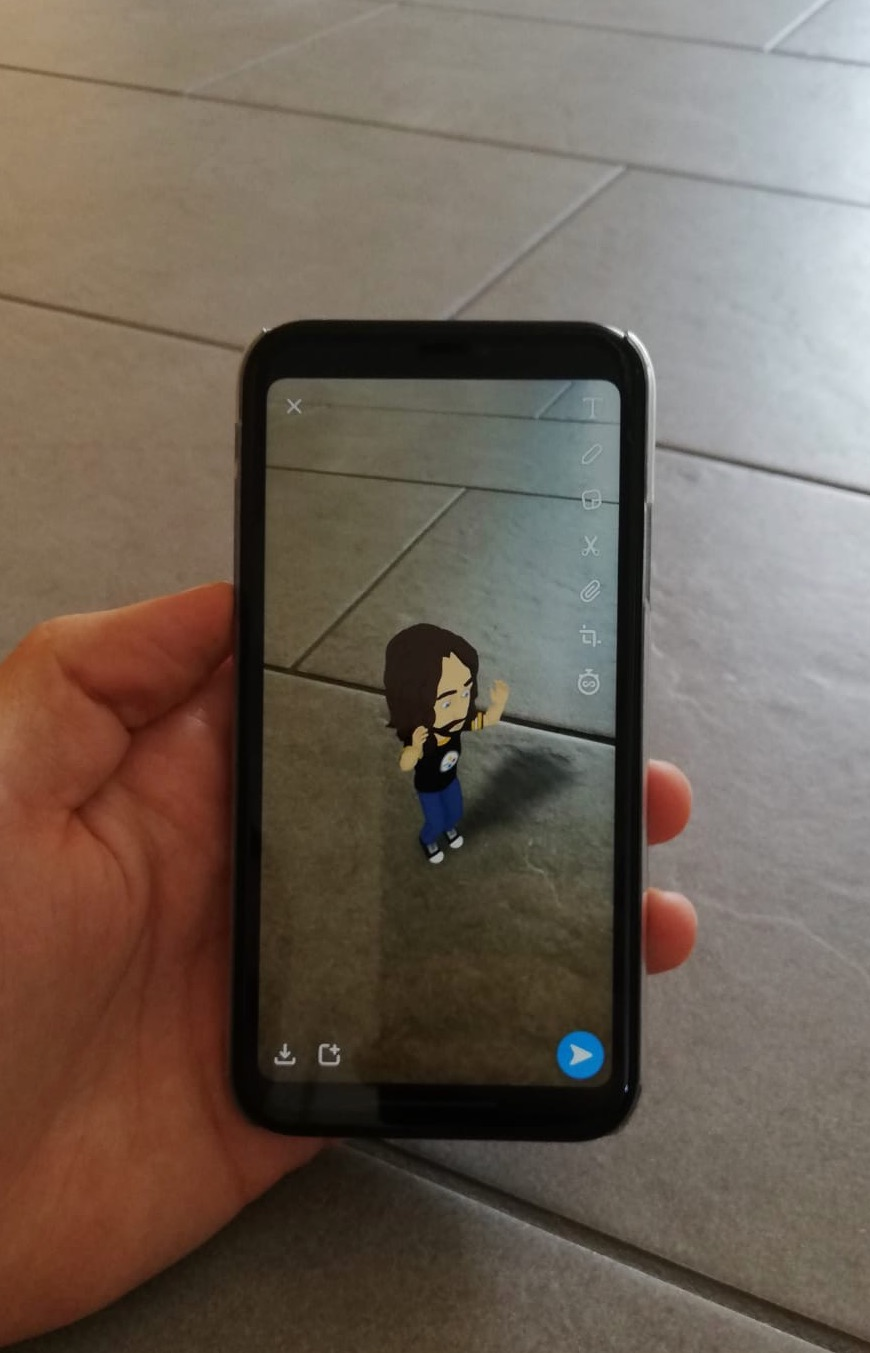
\includegraphics[width=6cm,height=6cm,keepaspectratio]{2Grundlagen/Bilder/snapchatAR.jpeg}
    \caption{Mobile-AR in Snapchat}
    \label{pic:snapchatAR}
\end{figure}
\pagebreak
\subsection*{Smart-Brillen AR}
\label{sec:smart-glasses}
Unter Smart- oder Datenbrillen und Smart Glasses wird ein Konstrukt verstanden, das eine Brille mit einem tragbaren Minicomputer verwirklicht. 
Dabei werden Informationen über kleinste Monitore oder Prismen ausgegeben und dem Nutzer zusätzlich in das Sichtfeld projiziert. Im Gegensatz
zur mobilen \acs{AR} hat der Nutzer kein Gerät in der Hand und ist somit in seiner Bewegung weniger eingeschränkt und flexibler. 
\\ 
\linebreak
Die Technologie der Smart-Brillen ist ein ähnliches Konzept zu der \acs{VR}-Brille, allerdings befindet sich die Smart-Brille für den 
öffentlichen Gebrauch noch in der Entwicklungsphase, da nur bedingte Funktionen möglich sind und die Kosten für den Normalverbraucher nur 
bedingt tragbar erscheinen. Mit der überarbeiteten Version der \textit{HoloLens 2} von Microsoft ist eine deutlich komfortablere und für 
den alltäglichen Gebrauch geeigneteren Ausführung entwickelt worden, die im Vergleich zum Vorgängermodell deutlich praktischer, leichter und handlicher ist. 
Das Design der Datenbrille ist von einer normalen Brille noch weit entfernt, ermöglicht mittlerweile aber das 
uneingeschränkte Sehen und Wahrnehmen der Umgebung. Die Bedienung des Geräts basiert auf schon vorhandenen Möglichkeiten die bereits in anderen 
Geräten Anwendung finden. Darunter gibt es am Gerät angebrachte Touchsensoren, Handbewegungen und -gesten und Eye-Tracking. 
\begin{figure}[hbt!]
    \centering
    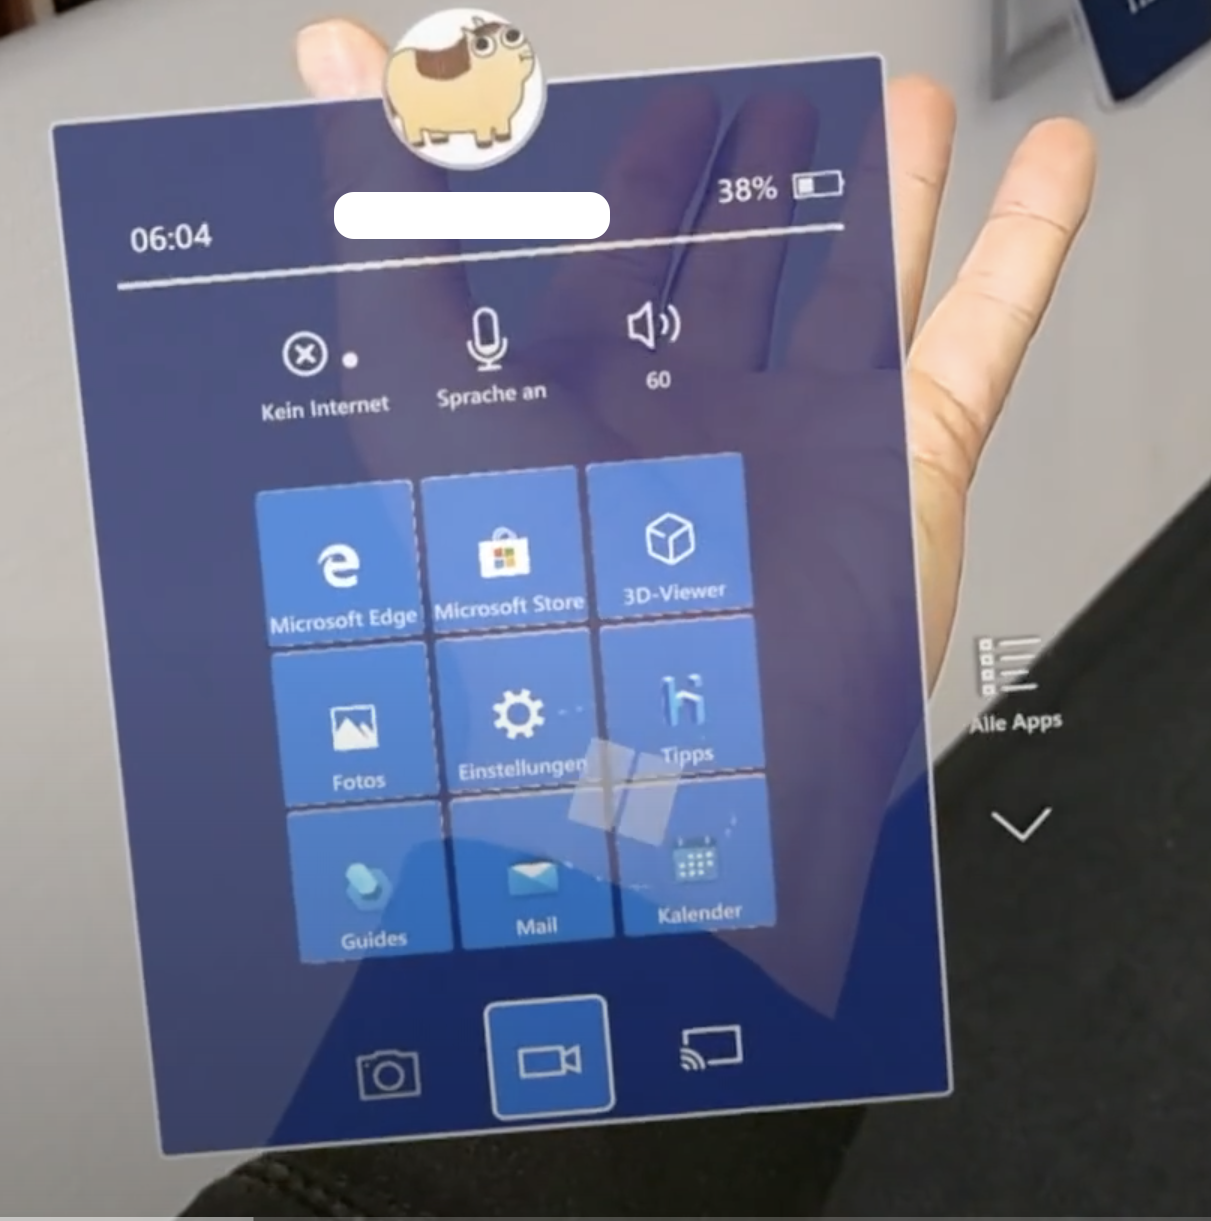
\includegraphics[width=10cm,height=7.5cm,keepaspectratio]{2Grundlagen/Bilder/smartglassAW.png}
    \caption{Test der HoloLens 2}
    \label{pic:testholo}
\end{figure}
\\ 
\linebreak %komfortables und
Speziell im industriellen Bezug bieten die neuentwickelten Brillen ein akzeptables Gewicht, sodass diese ohne große 
Probleme dauerhaft tragbar sind und den Mitarbeiter bei seiner Arbeit nicht übermäßig einschränken.
\\ 
\linebreak
Die Programmierung solcher \acs{AR}-Brillen laufen häufig über eigene \acs{SDK}s und plattformunabhängige Laufzeit- und 
Entwicklungsumgebungen, z.B. Unity oder Unreal Engine. Diese gelten als führende Produkte im Bereich der 3D-Echtzeitdarstellung.
Ein marktführendes Produkt ist unter anderem die Microsoft HoloLens 2, die der folgenden Abbildung zu entnehmen ist. 
\begin{figure}[hbt!]
    \centering
    \subfigure[Google Glass 2]{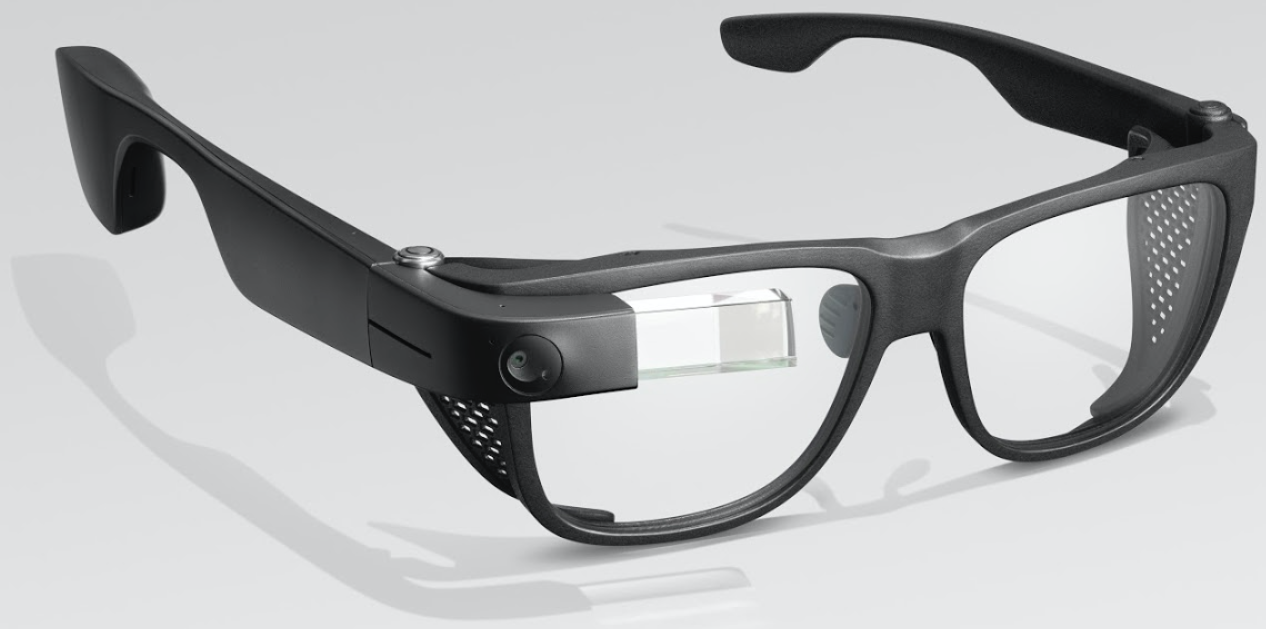
\includegraphics[width=7.5cm,height=5cm,keepaspectratio]{2Grundlagen/Bilder/googleglass.png}}
    \subfigure[HoloLens 2]{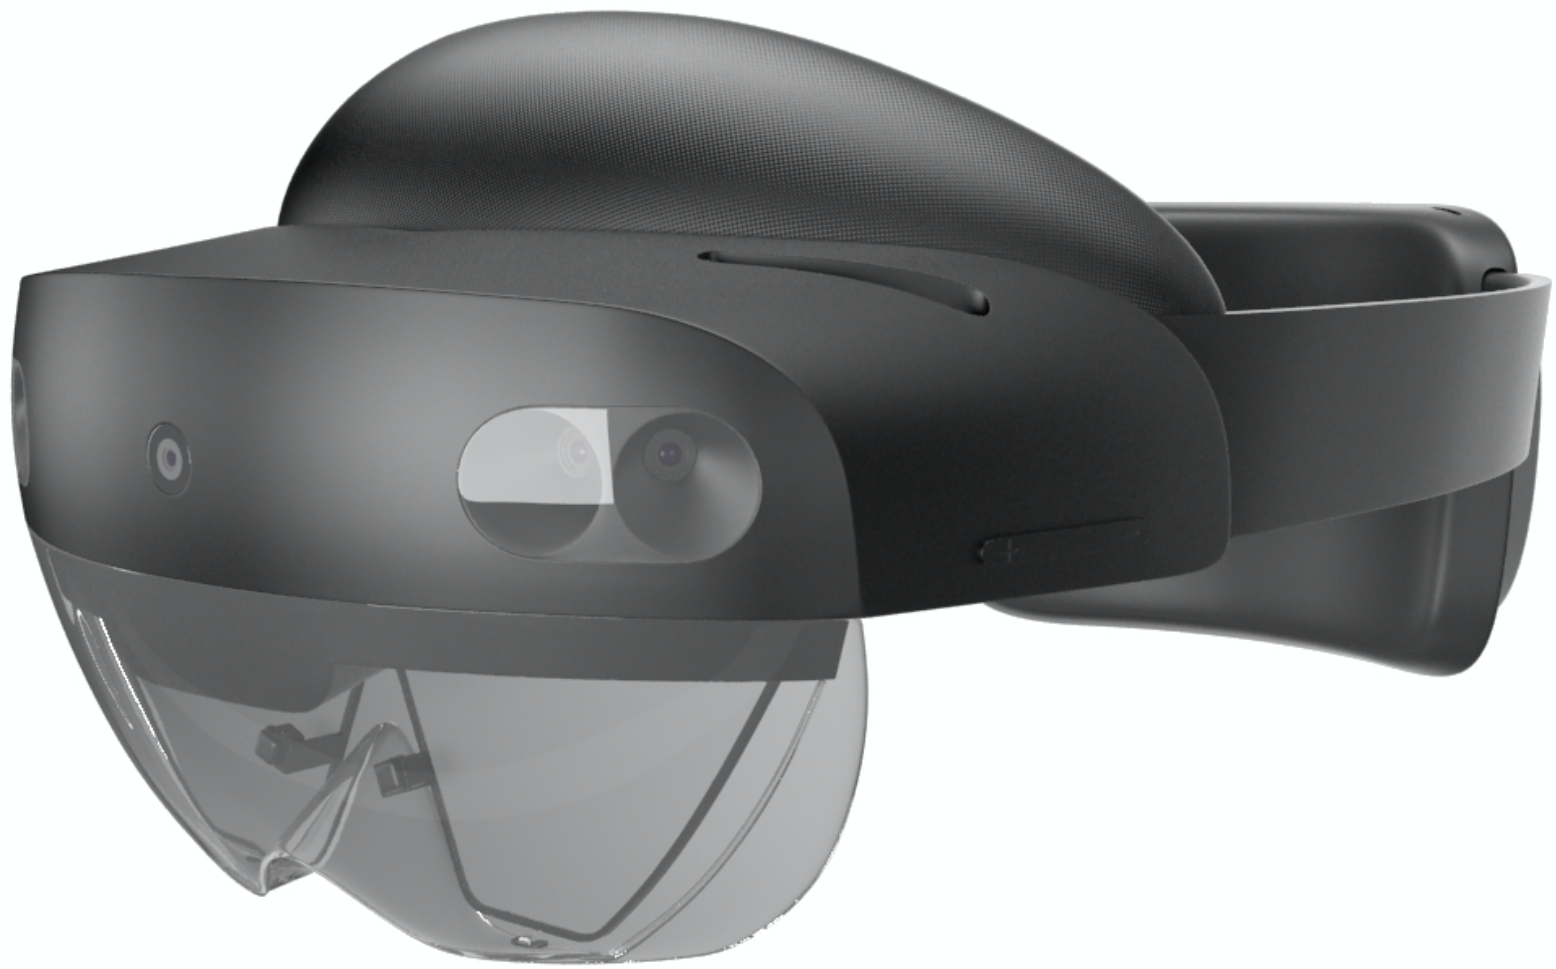
\includegraphics[width=7.5cm,height=5cm,keepaspectratio]{2Grundlagen/Bilder/hololensside.png}}
    \caption{Datenbrillen (\acs{HMD})}
    \label{pic:datenbrillen}
\end{figure}
\\ 
\linebreak
Eine große Herausforderung der \acl{AR} ist die Bestimmung der Position, in der Daten und Objekte projiziert werden. Auf die 
Ansätze, diese Herausforderung zu bewältigen, wird in folgendem Abschnitt \ref{sec:posi} eingegangen.
\subsection{Positionsbestimmung}
\label{sec:posi}
Um ein digitales Objekt als Overlay dem Kamera-Live-Bild hinzuzufügen, werden genauestens definierte Positionen benötigt. Diese Positionen 
können durch unterschiedliche Ansätze ermittelt werden. Je nach Anwendungsfall, z.B. als Navigation, Routenplaner oder Google Maps 
\textit{„Live View“} \cite{googleliveview.2019a}, reicht eine etwas ungenauere Positionsbestimmung per \acs{GPS}, da in Relation zur 
realen Welt eine Abweichung um Zentimeter oder wenige Meter nicht von Belang ist. Bei Positionsbestimmungen auf kleinstem Raum ist eine 
genaue Lokalisierung wichtig und basiert auf einem deutlich präziseren Ansatz. 
\\ 
Welche oben genannten Ansätze es gibt und welche Unterschiede zu beachten sind, wird in Folgendem näher erläutert. 
\subsubsection*{Marker-basierte Positionsbestimmung}
Speziell bei der Marker-basierten Positionsbestimmung gibt es verschiedene Möglichkeiten den Marker zu gestalten. Es können 
Binär- oder QR-Codes als Markierung verwendet werden, ein Beispiel eines solchen Codes ist der Abbildung \ref{pic:markerARpos} zu entnehmen. 
Diese Codes sind meistens quadratisch und haben ein eindeutiges Zeichen in der Mitte. Um die Rechenzeit gering zu halten gibt es einfache Muster, 
wie die Abbildung \ref{pic:markerARpos} zeigt.
\begin{figure}[hbt!]
    \centering
    
\includegraphics[width=5cm,height=5cm,keepaspectratio]{2Grundlagen/Bilder/bildmarkerAR.png}
    \caption{Marker-basierte Augmented Reality Positionsbestimmung}
    \label{pic:markerARpos}
\end{figure}
\pagebreak
\\ 
\linebreak
Neben der einfachen Markierungserkennung gibt es eine weiterentwickelte Möglichkeit der Bild- sowie der Objekterkennung. Diese sind Ansätze 
die grundlegend auf dem Ausgangspunkt des Binär-Code-Verfahrens aufbauen. Eine detailliertere Erläuterung der soeben genannten 
Erkennungsmöglichkeiten findet im Rahmen dieser Arbeit nicht statt, allerdings wird allgemein kurz auf die Funktionsweise einer 
Marker-basierten Positionsbestimmung eingegangen.
\\ 
Durch ein Kamerabild wird nach einem vordefinierten Marker, bzw. nach einer festgelegten Markierung gesucht. Ist diese mit der Kamera erfasst, 
wird die Markierung durch Bildverarbeitungsalgorithmen und bestimmter Filterung eindeutig identifiziert. Mit den gewonnen Informationen und 
der Übereinstimmung des angegebenen Codes wird die Position, sowie die Orientierung des Markers berechnet. Mit den Angaben der Lage und 
Orientierung wird auf der Markierung das anzuzeigende digitale Objekt generiert und als Overlay über dem Kamerabild angezeigt. Die Markierung 
dient sozusagen als Grundlage um den digitalen Gegenstand überhaupt anzeigen zu können.
\\ 
Da der Marker immer im Blickfeld der Kamera sein muss, um das virtuelle Objekt anzuzeigen, bringt diese Art der Positionsbestimmung eine 
enorme Einschränkung mit sich, die in diesem Bezug unumgänglich ist. 
\\ 
\linebreak
Ein weiterer Ansatz der Positionsbestimmung ist als Überbegriff das Gegenstück zur oben aufgeführten Lokalisierung von Markern, die 
sogenannte Marker-unabhängige Positionsbestimmung, welche ebenso verschiedene Ausführungen vorweist. 
\subsubsection*{\acs{GPS}-basierte Positionsbestimmung}
Die Methode des \acs{GPS}-basierten Positionsbestimmungsverfahren verwendet hauptsächlich die Koordinaten der realen Welt. In Zusammenarbeit 
mit zusätzlichen im Anwendungsgerät verbauten internen Sensoren, bspw. Positions-, Geschwindigkeits- und Beschleunigungssensoren und Teile des 
\ac{INS}, z.B. dem Gyroskop, kann diese Art der Positionsbestimmung optimal Anwendung finden. Allerdings werden dabei deutlich mehr Komponenten
benötigt und ist deutlich komplexer umzusetzen, als ein markerbasiertes System. 
\\ 
Bei einem Anwendungsfall von \acs{GPS}-basierter Positionsbestimmung geht es meist um Routenplaner, Navigation oder Szenarien die sich 
auf offenen Flächen abspielen, da im Gegensatz zu Marker-basierten Anwendungen das Größenverhältnis deutliche Unterschiede vorweist. 
Der Benutzer ist nicht auf einen bestimmten Bezirk beschränkt und ist nicht auf die millimetergenauer Darstellung angewiesen.
\\ 
\linebreak
Eine Alternative zu \acs{GPS} ist die Anwendung des \acs{SLAM}-Verfahrens. Dabei wird eine virtuelle Karte, bzw. ein geometrischen Modell der 
Umgebung erstellt. Wichtige Grundlagen zum Erzeugen eines solchen Modells sind eigenständig gefundene Landmarken die gleichzeitig 
lokalisiert werden. Darauf folgt ein Vergleich der Pose, der Position des Geräts und der geschätzten Karteninformationen aus dem Scan der 
Umgebung. 
Damit sind im erweiterten Sinne Marker geschaffen, die Anhaltspunkte für \acl{AR}-Interaktionen schaffen.
\\ 
In Kapitel \ref{chap:SLAM} wird die Thematik des \acs{SLAM}-Verfahrens erläutert. 

\subsection{Augmented Reality in der Industrie}
\label{sec:ARIndustrie}
Das weit gefächerte Portfolio der \acl{AR} umfasst viele Anwendungsbereiche und Fachgebiete. Selbst dem übergeordneten Bereich der Industrie 
gibt es viele verschiedene Einsatzgebiete. Aus den vielen Möglichkeiten der Anwendung haben sich über die Jahre der Entwicklung der Technologie 
einige Gebiete in der Industrie herauskristallisiert, die besonders großen Nutzen davon haben. \cite{einsatzgebietear.2017a} In den Bereichen 
Instandhaltung und Wartung, Betrieb und Training ist \acl{AR} auf bestem Wege, fester Bestandteil des Alltags zu werden. Bei dieser Betrachtung 
ist es sinnvoll, sich auf die damit einhergehenden Lösungen, die Reduktion der Kosten und dem Zeitaufwand, sowie die Verbesserung 
der Sicherheit, zu fokussieren. \cite{studieptc.2020j} 
\\ 
\linebreak
Bei einer Wartung oder Reparatur einer Maschine sind notwendige Informationen direkt greifbar und werden Schritt für Schritt angezeigt, sodass 
in bestimmten Situationen selbst ein Leihe die Anweisungen befolgen könnte. So werden zusätzliche Recherchearbeiten oder Unklarheiten über 
Vorgänge aus dem Weg geräumt. Ein Mitarbeiter kann so mit einem Tablet oder einer Smart-Glas Anweisungen visuell auf die realen Maschinen 
projizieren und Arbeitsschritte im Sichtfeld anzeigen lassen. Ebenso geht dieser Vorgang auch bei der Produktion von Bauteilen o.ä., indem 
eine \acs{AR}-Anwendung Anweisungen und Prozessschritte, z.B. auf das Werkstück oder Produkt, projiziert.
\\ 
Die Inbetriebnahme oder Bedienung einer komplexen Anlage oder Maschine ist nach herkömmlichen Standard enorm zeitintensiv und dadurch können
zusätzlich viele Fragen aufkommen, die meist den Prozess noch länger gestalten als vorgesehen. \acs{AR}-Anwendungen können 
Bedienungsanleitung oder -hilfen digitalisiert, indem Informationen, Inhalte oder Bedienelemente durch \acl{AR} auf der Anlage platziert werden. 
\\ 
In Fortbildungen, Schulungen oder Einarbeitungen in neue Geräte kann \acs{AR} durchaus von großem Vorteil sein. Mit wenig Aufwand, einem 
effektiveren Training können Schulungen interaktiver und vor allem sicherer abgehalten werden. Durch die Visualisierung der Trainings- und 
Schulungsinhalten verbessert sich der Lernprozess und damit wird auch die Nutzung der Maschinen verständlicher. \cite{einsatzgebietear.2017a}